

%col{x}{y}{z} respresents the color for ball z from matrix x at stage y (matrix x, stage y, ball z)
 
\definecolor{light-gray}{gray}{0.6}
\begin{figure}

  \begin{subfigure}{\textwidth}
  \centering
  %\begin{subfigure}[b]{0.15\textwidth}
    \begin{tikzpicture}[scale=1.0,auto,swap]

    % the two brain figures on top
    \node (upper_brain) at (0,1.5) { \includegraphics*[scale=\scaleBrainImg,trim=0 0 240 0]{\snapLocationAD/stage_8.eps}};
    \node (lower_brain) at (0,-1.5) { \includegraphics*[scale=\scaleBrainImg,trim=240 0 0 0]{\snapLocationAD/stage_8.eps}};
    \node[above=0cm of upper_brain] (stage) {Stage 8};
    % the balls
    
    \end{tikzpicture}
  %\end{subfigure}
  % next subfigure
  \hspace{-1.5em}
  ~
  %\begin{subfigure}[b]{0.15\textwidth}
    \begin{tikzpicture}[scale=1.0,auto,swap]

    % the two brain figures on top
    \node (upper_brain) at (0,1.5) { \includegraphics*[scale=\scaleBrainImg,trim=0 0 240 0]{\snapLocationAD/stage_16.eps}};
    \node (lower_brain) at (0,-1.5) { \includegraphics*[scale=\scaleBrainImg,trim=240 0 0 0]{\snapLocationAD/stage_16.eps}};
    \node[above=0cm of upper_brain] (stage) {Stage 16};
    % the balls
    
    \end{tikzpicture}
  %\end{subfigure}
  % next subfigure
  \hspace{-1.5em}
  ~
  %\begin{subfigure}[b]{0.15\textwidth}
    \begin{tikzpicture}[scale=1.0,auto,swap]

    % the two brain figures on top
    \node (upper_brain) at (0,1.5) { \includegraphics*[scale=\scaleBrainImg,trim=0 0 240 0]{\snapLocationAD/stage_24.eps}};
    \node (lower_brain) at (0,-1.5) { \includegraphics*[scale=\scaleBrainImg,trim=240 0 0 0]{\snapLocationAD/stage_24.eps}};
    \node[above=0cm of upper_brain] (stage) {Stage 24};
    % the balls
    
    \end{tikzpicture}
  %\end{subfigure}
  % next subfigure
  \hspace{-1.5em}
  ~
  %\begin{subfigure}[b]{0.15\textwidth}
    \begin{tikzpicture}[scale=1.0,auto,swap]

    % the two brain figures on top
    \node (upper_brain) at (0,1.5) { \includegraphics*[scale=\scaleBrainImg,trim=0 0 240 0]{\snapLocationAD/stage_32.eps}};
    \node (lower_brain) at (0,-1.5) { \includegraphics*[scale=\scaleBrainImg,trim=240 0 0 0]{\snapLocationAD/stage_32.eps}};
    \node[above=0cm of upper_brain] (stage) {Stage 32};
    % the balls
    
    \end{tikzpicture}
  %\end{subfigure}
  % next subfigure
  \hspace{-1.5em}
  ~
  %\begin{subfigure}[b]{0.15\textwidth}
    \begin{tikzpicture}[scale=1.0,auto,swap]

    % the two brain figures on top
    \node (upper_brain) at (0,1.5) { \includegraphics*[scale=\scaleBrainImg,trim=0 0 240 0]{\snapLocationAD/stage_40.eps}};
    \node (lower_brain) at (0,-1.5) { \includegraphics*[scale=\scaleBrainImg,trim=240 0 0 0]{\snapLocationAD/stage_40.eps}};
    \node[above=0cm of upper_brain] (stage) {Stage 40};
    % the balls
    
    \end{tikzpicture}
  %\end{subfigure}
  % next subfigure
  \hspace{-1.5em}
  ~
  \hspace{1em}
  % the red-to-yellow gradient on the right
  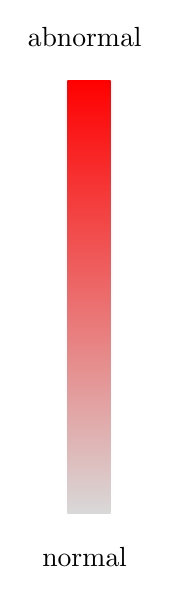
\begin{tikzpicture}[scale=1.1,auto,swap]
    \shade[top color=red,bottom color=gray!30] (0,0) rectangle (0.5,5);
    \node[inner sep=0] (corr_text) at (0.2,5.5) {abnormal};
    \node[inner sep=0] (corr_text) at (0.2,-0.5) {normal};
  \end{tikzpicture}
  \caption{}
  \label{fig:SnapEBMADa}
  \end{subfigure}
  
  \begin{subfigure}{1\textwidth}
  \centering
  \includegraphics[scale=0.6]{\snapLocationAD/../patientStages.eps}
  \caption{}
  \label{fig:SnapEBMADb}
  \end{subfigure}

  \captionSnapEBMAD
  
\end{figure}


